\documentclass[9pt,twocolumn,twoside]{../../styles/osajnl}
\usepackage{fancyvrb}
\journal{i524} 

\title{Flight Data Analysis Using Big Data Tools}

\author[1,*]{Anvesh Nayan Lingampalli}

\affil[1]{School of Informatics and Computing, Bloomington, IN 47408, U.S.A.}

\affil[*]{Corresponding authors:anveling@indiana.edu}

\dates{project-S17-IR-2016, \today}

\ociscodes{Apache, Hive, Ansible, Pig, I524}

\doi{Report: \url{https://github.com/cloudmesh/sp17-i524/tree/master/project/S17-IR-2016/report/report.pdf}\\
Code: \url{https://github.com/cloudmesh/sp17-i524/tree/master/project/S17-IR-2016/code}


\begin{abstract}
Analysis of flight data provides insights on the United States of
America's Airline data by using Hadoop in the cloud environment. The
On-time performance of flights operated by large air carriers are
tracked and made as a report, Air Travel Consumer Report, which is a
big data set. Hive component of Hadoop ecosystem, is utilized to
process the big data in distributed environment. Efficient accessing
and processing of the user queries is acheived by this analysis on
flight data.
\newline
\end{abstract}

\setboolean{displaycopyright}{true}

\begin{document}

\maketitle

\section{Introduction}

Real world data is large and growing exponentially from several
years. This data can be in structured or unstructured format which is
popularly known as Big Data\cite{bigdata}. Aviation industry manages
enormous amount of data, which consists of the information regarding
the delayed, cancelled, diverted or on-time flights by large
air-carriers\cite{aviationanalysis}. This is essentially a big-data
set, where statistics are publicly available as the Air Travel
Consumer Report.

Access to multiple clouds is provided by a cloud manager known as
Cloudmesh Client\cite{cloudmesh}. With the help of this cloud manager,
Hadoop cluster is built with neccessary add-ons such as Apache
Spark\cite{spark}, Hive\cite{hive}, Pig\cite{pig}. Cloudmesh Client is
also used in the deployment of the cluster on various clouds such as
Chameleon cloud\cite{chameleon} or Jetstream\cite{jetstream}
cloud. Deployment part is automated with the help of
ansible\cite{ansible} scripts where data is extraced, stored and
analysed automatically to produce the results.

Big Data analysis of this data will provide a
consistent understanding and importance of the given data. With 35
million flight departures per year, data is critically important for
any planning decision made by airlines and airports. The results of
analysis has benefits which can help airline operations to predict and
reduce redundance\cite{bigdatainaviation}.

\section{Infrastructure}

Cloudmesh client and Chameleon cloud forms the infrastructure of this
analysis project.

Cloudmesh client is a toolkit which provides a client interface for
accessing different clouds and clusters. It includes a commandline
interface to provide abstraction from backend databases. Simplicity is
one of the key and powerful features of the cloudmesh client. It makes
switching between various clouds easy by providing a convenient
programmable interface.

Chameleon cloud is a large scale platform which is an open research
community for development of programmable cloud services. It provides
wide range of services such as Infrastructure-as-a-service,
platform-as-a-service and delivery of high functioning cloud
environment.

\section{Deployment tools}

\subsection{Ansible}

Ansible is an open source software that provides automation for
configuration management and application deployment. It facilitates a
simple automation platform that makes the application easier to
deploy. It also handles ad-hoc task execution and multinode
orchestration. Ansible is a software which has an agent-less
architecture. This is because there are no deamon processes running in
the background.  Components of Ansible comprises of modules,
playbooks,inventory and ansible towers.  Modules can control system
resources like services, packages, or files. Inventory is
configuration file that reflects the nodes that are available for
access. Nodes are represented by hostnames or IP addresses. Playbooks
are Ansible's configuration, deployment and orchestration
language. These are in the YAML format. Playbooks are generally used
to manage configurations and deployment on remote machines. Ansible
tower makes Ansible a center for automating tasks by providing a web
based console\cite{ansible-tutorial}.

\begin{figure}[ht]
  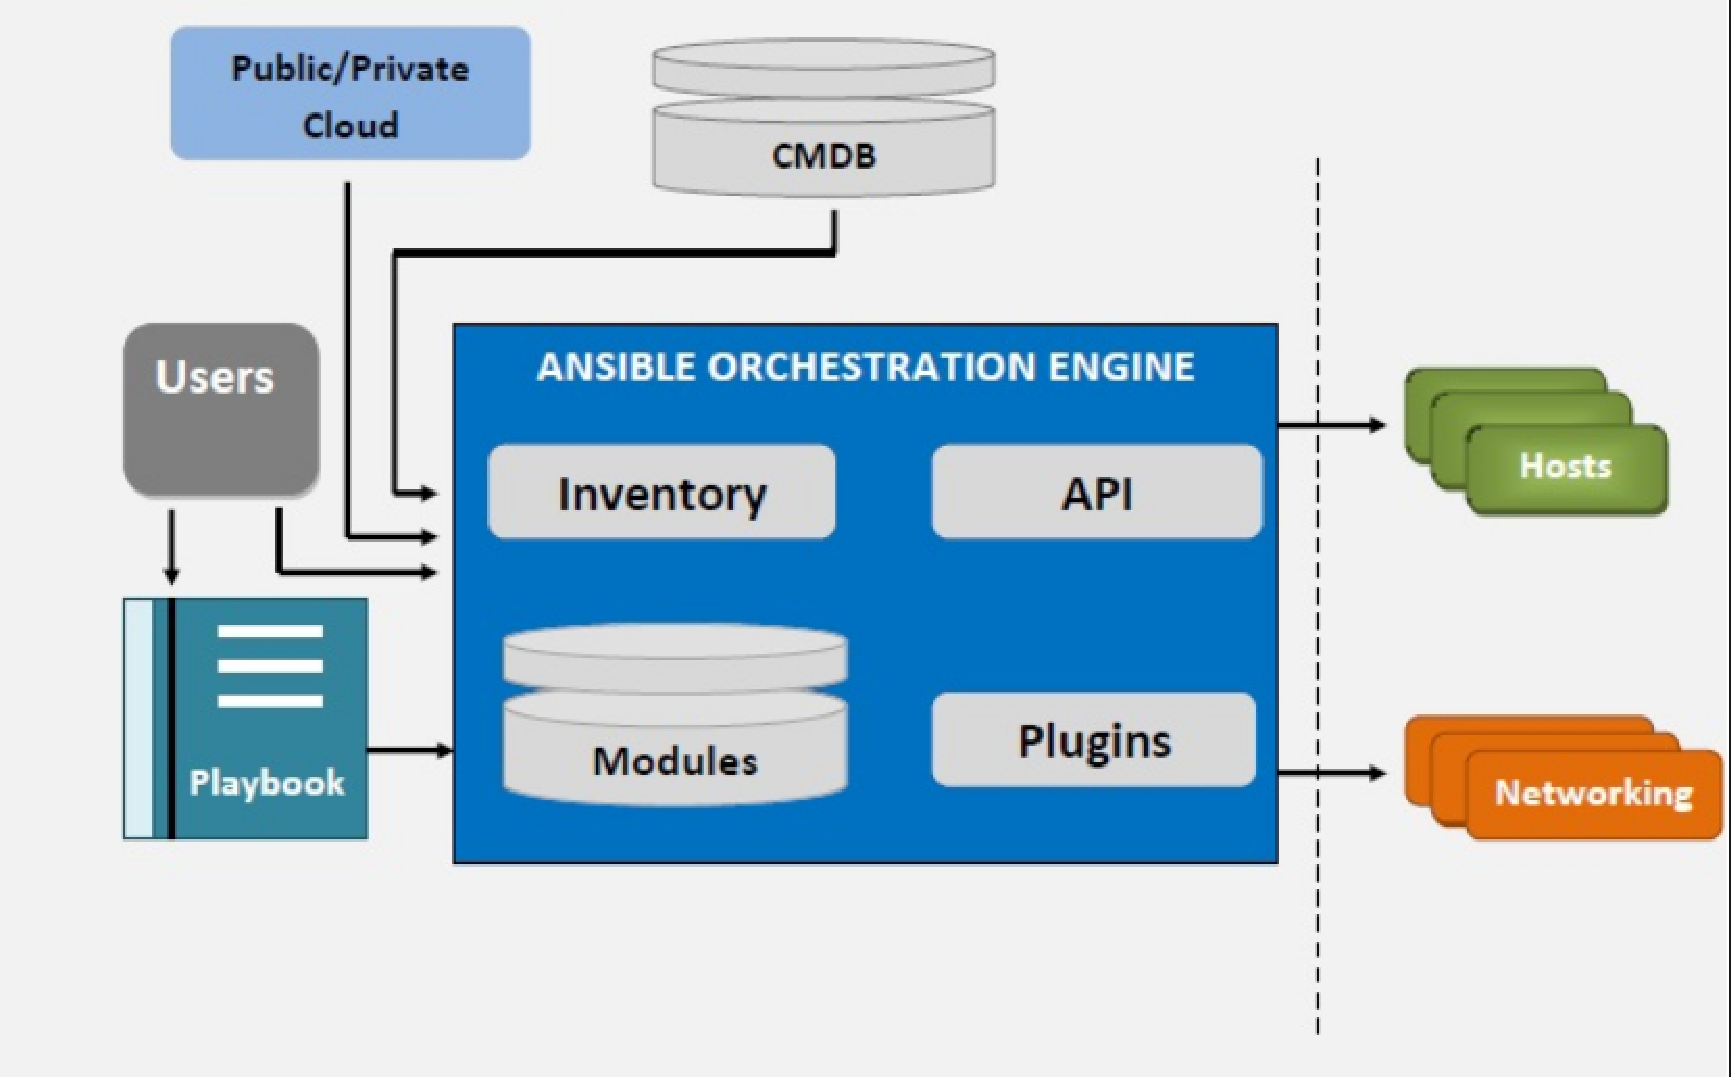
\includegraphics[width= \linewidth, height =
    2.5in]{images/ansible_architecture.pdf}
  \caption{Architecture of Ansible}\cite{ansible-architecture}
\end{figure}

\section{Analysis tools}

\subsection{Apache Hive}

Hive is one of the ecosystems in Hadoop\cite{hadoop} framework which is built to
analyze the data on hadoop cluster. Syntax of Hive is based on SQL\cite{sql},
which is also known as HiveQL. MySQL or PostGreSQL\cite{postgresql} can be used for
implementation of the queries. Hive provides tools which enable easy
data extraction, transformation and data loading. Files can be stored
in Hadoop Distributed File System(HDFS)\cite{hdfs} and accessed by Hive
efficiently.

Schema of the Hive tables is stored in Hive Metastore. Metastore holds
the information about tabes and partitions which are present in the
data warehouse. In Hive the default Metastore is DerBy Database, which
is a relational database management system provided by Apache
Software.  There are two components of Hive, HCatalog and
WebHCat. HCatalog is a storage management layer for Hadoop which
provides data processing tools such as Pig and MapReduce. WebHCat
provides a service that is used to run Hadoop MapReduce, Pig, Hive
jobs using REST interface\cite{hive-website}.

\begin{figure}[ht]
  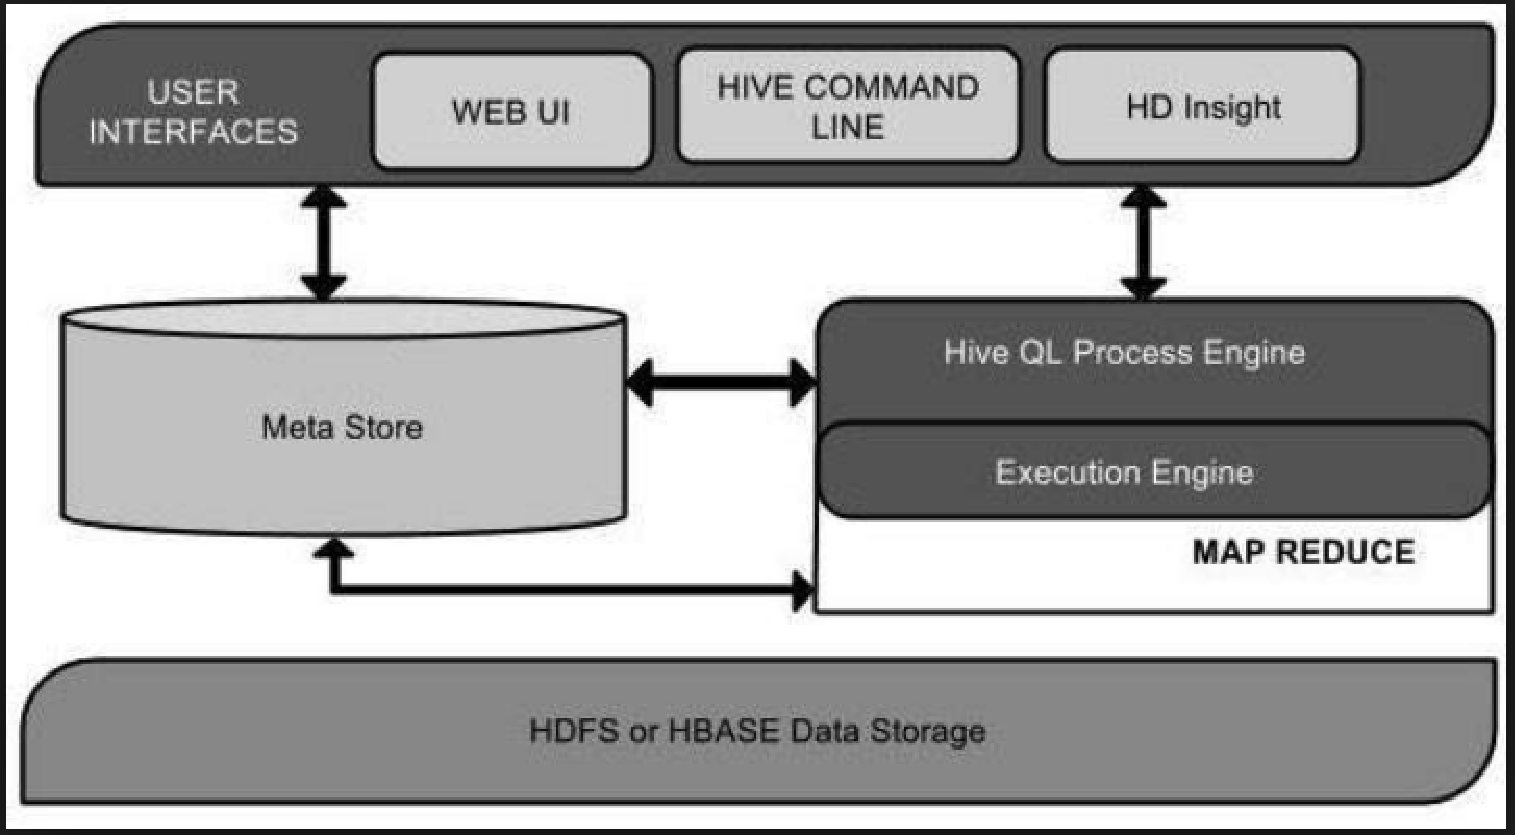
\includegraphics[width= \linewidth, height =
    2.5in]{images/hive_architecture.pdf}
  \caption{Apache Hive Architecture}\cite{hive-architecture}
\end{figure}

Hive's SQL provides the basic SQL operations, such as,
\begin{itemize}
  
\item Filtering the rows from the table using WHERE clause.
  
\item Selecting columns from table using SELECT clause.
  
\item Joining two tables
  
\item Aggregations of the data using 'group by' clause.

\item Storing the results in a hdfs directory.

\end{itemize}

\subsection{Hadoop Distributed File System}

Hadoop Distributed File System provides a distributed file data
storage system which spans large clusters of servers. It distributes
-the storage and computation across many servers which maintains
economy of the storage\cite{hdfs}.

The file system is designed to be fault-tolerant. When HDFS takes
data, the information is broken into pieces and distributed them to
different nodes in a cluster. This provides parallel processing on
clusters. MapReduce programming model is implemented when the
applications are executed. 

HDFS uses master/slave architecture, where each cluster consists of a
Namenode, which manages file system operations and supports Datanodes,
which manage data storage on individual compute nodes. Namenodes
monitor the Datanodes in creating, deleting and replicating data by
mapping them into data nodes.

\begin{figure}[ht]
  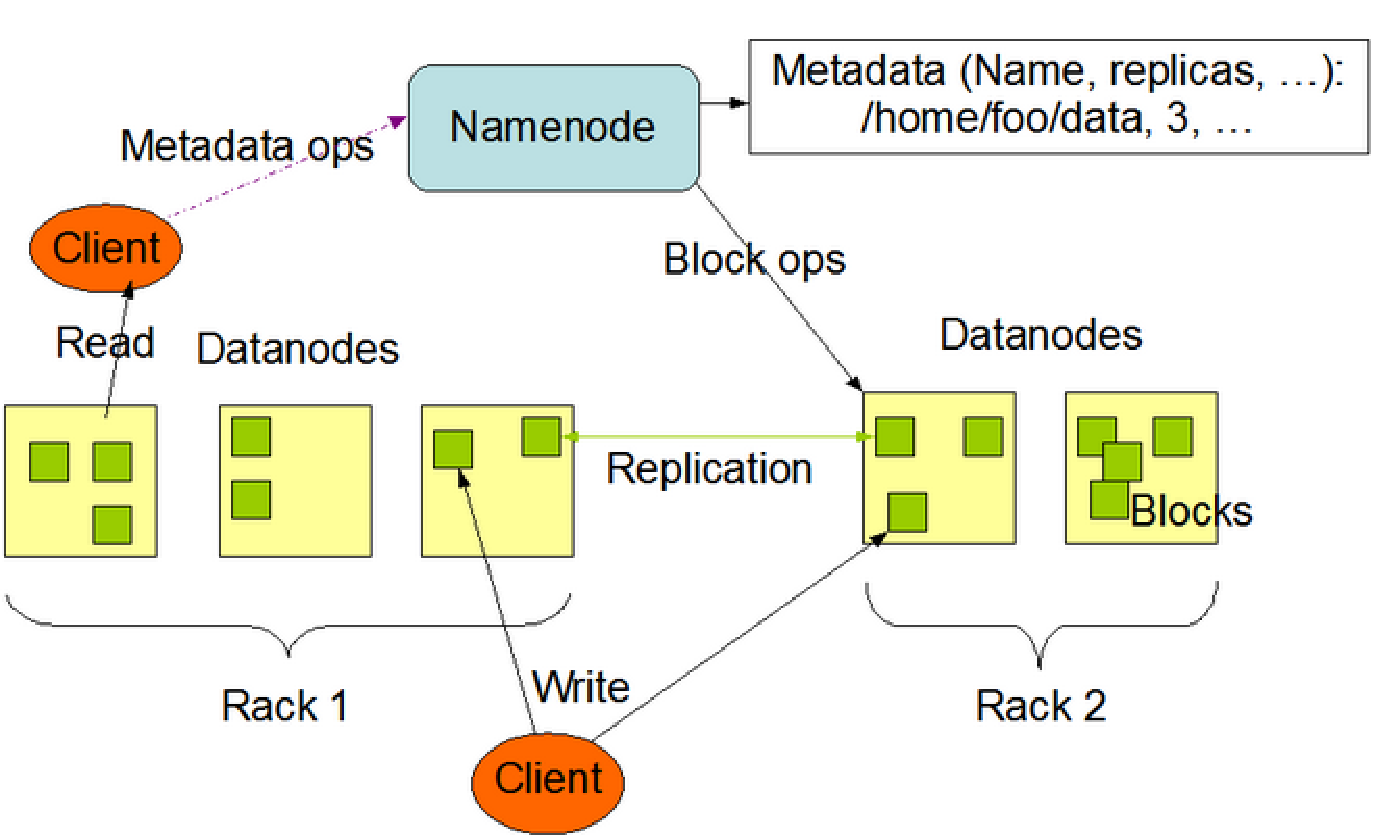
\includegraphics[width= \linewidth, height =
    2.5in]{images/hdfs_architecture.pdf}
  \caption{Architecture of Hadoop Distributed File
    System}\cite{hdfs-architecture}
\end{figure}

\section{Implementation}

Implementation of Hive to perform data analysis consists of the
following steps.
\begin{itemize}
  \item Virtual machines are created on Chameleon Cloud with the help
    of Cloudmesh Client.    
  \item Hadoop cluster is deployed on Chameleon cloud.
  \item Flight Data is loaded into HDFS.
  \item Data is then transfered to Hive tables.
  \item Finally, analysis is done on Hive tables using HiveQL, this
    can either be done using Hive interface or by installing
    PostgresQL interface.
\end{itemize}

\subsection{Analysis in Hive Query Language}
  The following are the queries in Hive QL, which are similar to SQL
  statements.
 
  What are the total number of flights which are cancelled?
  \begin{verbatim}

    SELECT year, month, count(cancelled) as Cancelled-flights
    FROM Airline
    WHERE cancelled = 1
    GROUP BY YEAR, MONTH
    ORDER BY YEAR, MONTH
    LIMIT 20
    
  \end{verbatim} 

  What are the total number of flights which are diverted?
  \begin{verbatim}

    SELECT year, count(diverted) as Diverted-flights
    FROM Airline
    WHERE diverted = 1
    GROUP BY month
    ORDER BY month
    LIMIT 10
    
  \end{verbatim}

  Similarly, analysis of the data is done where the queries are as follows.
  
  What is effect of flight distance on cancellations?
  
  What is the effect of flight distance on average departure delay?
  
  What is the monthly average departure delay?

  What is the yearly average departure delay?

\section{Technologies}

\begin{itemize}
\item Distributed Computation and Storage:- HDFS and Hive
\item Development:- PostgreSQL and Java
\item Deployment:- Ansible
\end{itemize}

\section{Benchmarking}

After the deployment stage, benchmarking is implemented. This process
is important as it evaluates the performance of the application and
the system. This project is implemented on the chameleon cloud and the
results are observed. Different cloud environments are used for
creting these benchmarks

Characteristics of Chameleon cloud on which the analysis is implemented are,

\begin{figure}[ht]
  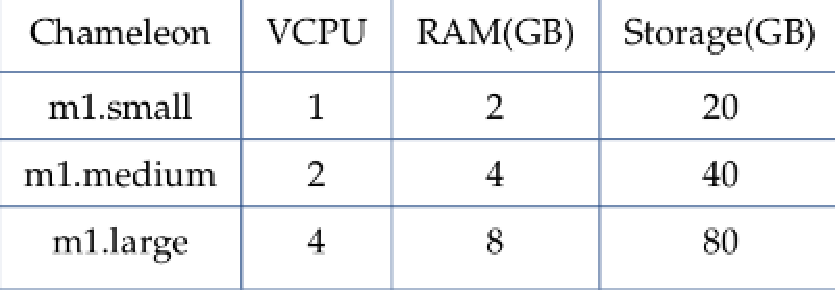
\includegraphics[width= \linewidth, height =
    1.5in]{images/chameleonfla.pdf}
  \caption{Different types of chameleon clouds}
\end{figure}

The following are the observations from the analysis on chameleon
cloud of different flavors.

\begin{figure}[htbp]
  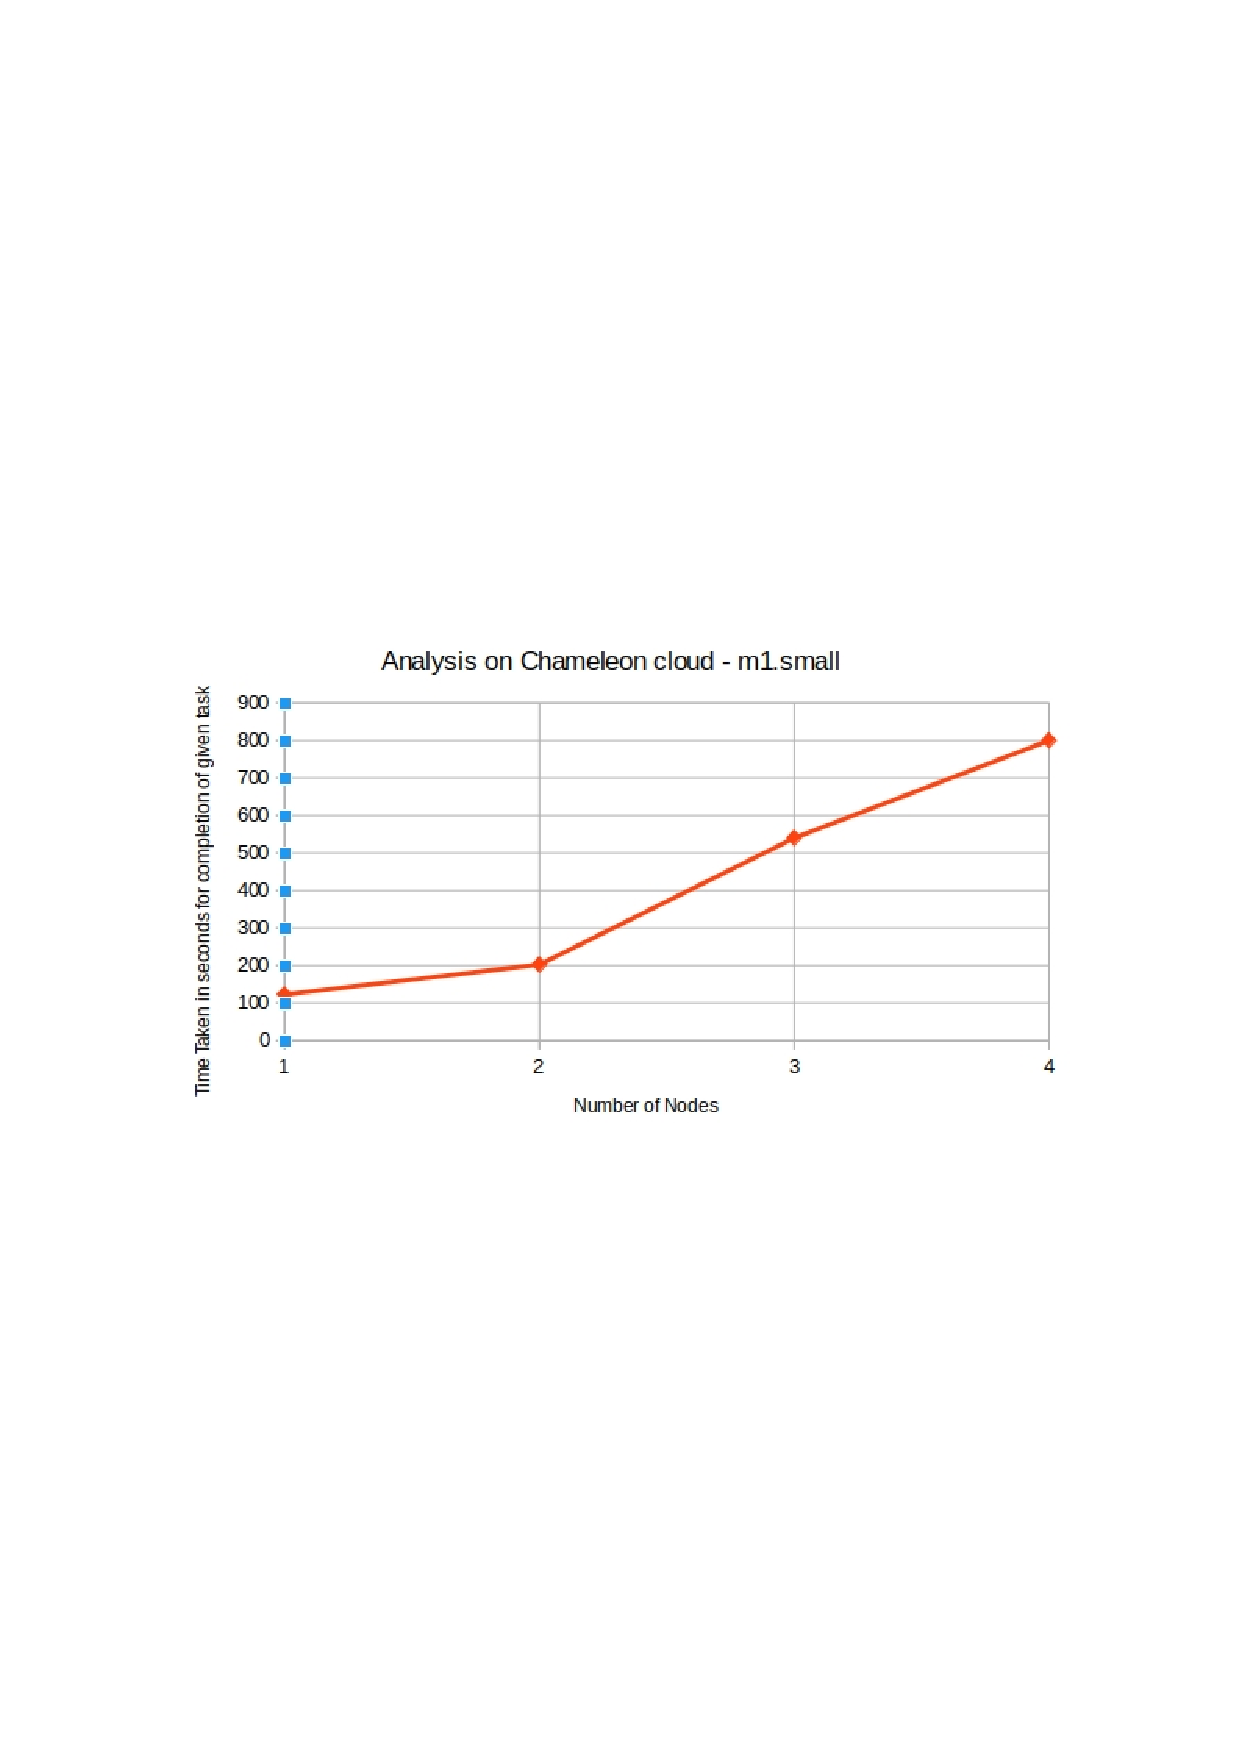
\includegraphics[width= \linewidth, height =
    2.5in]{images/m1small.pdf}
  \caption{Analysis time taken for a HiveQL-m1.small }
\end{figure}

These are the observed results when m1.small cloud is used for
analysis As the number of nodes in a cluster increase, the amount of
time the task takes to complete is increasing. This trend is also
observed when m1.medium and m1.large flavors of Chameleon cloud are
used.

\begin{figure}[htbp]
  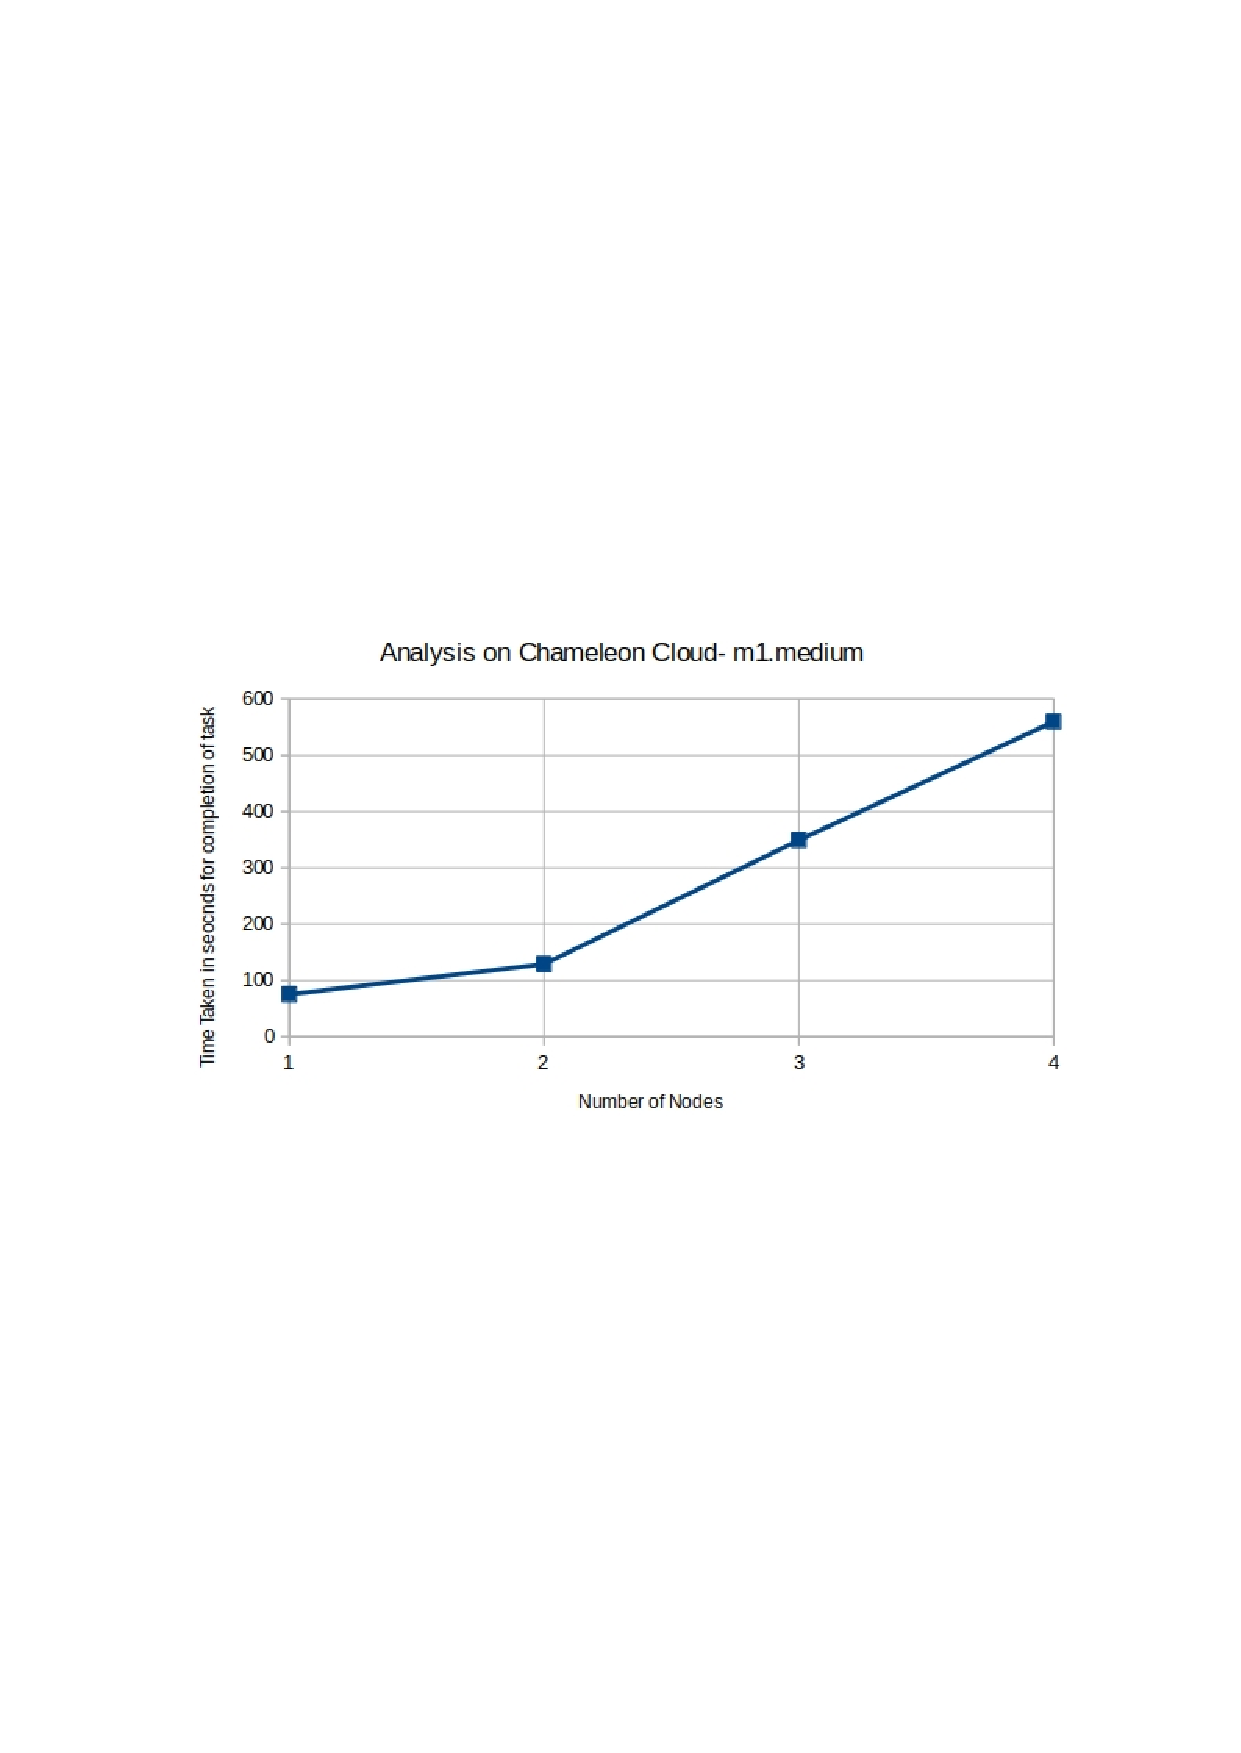
\includegraphics[width= \linewidth, height =
    2.5in]{images/m1medium.pdf}
  \caption{Analysis time taken for a HiveQL-m1.medium }
\end{figure}

\begin{figure}[htbp]
  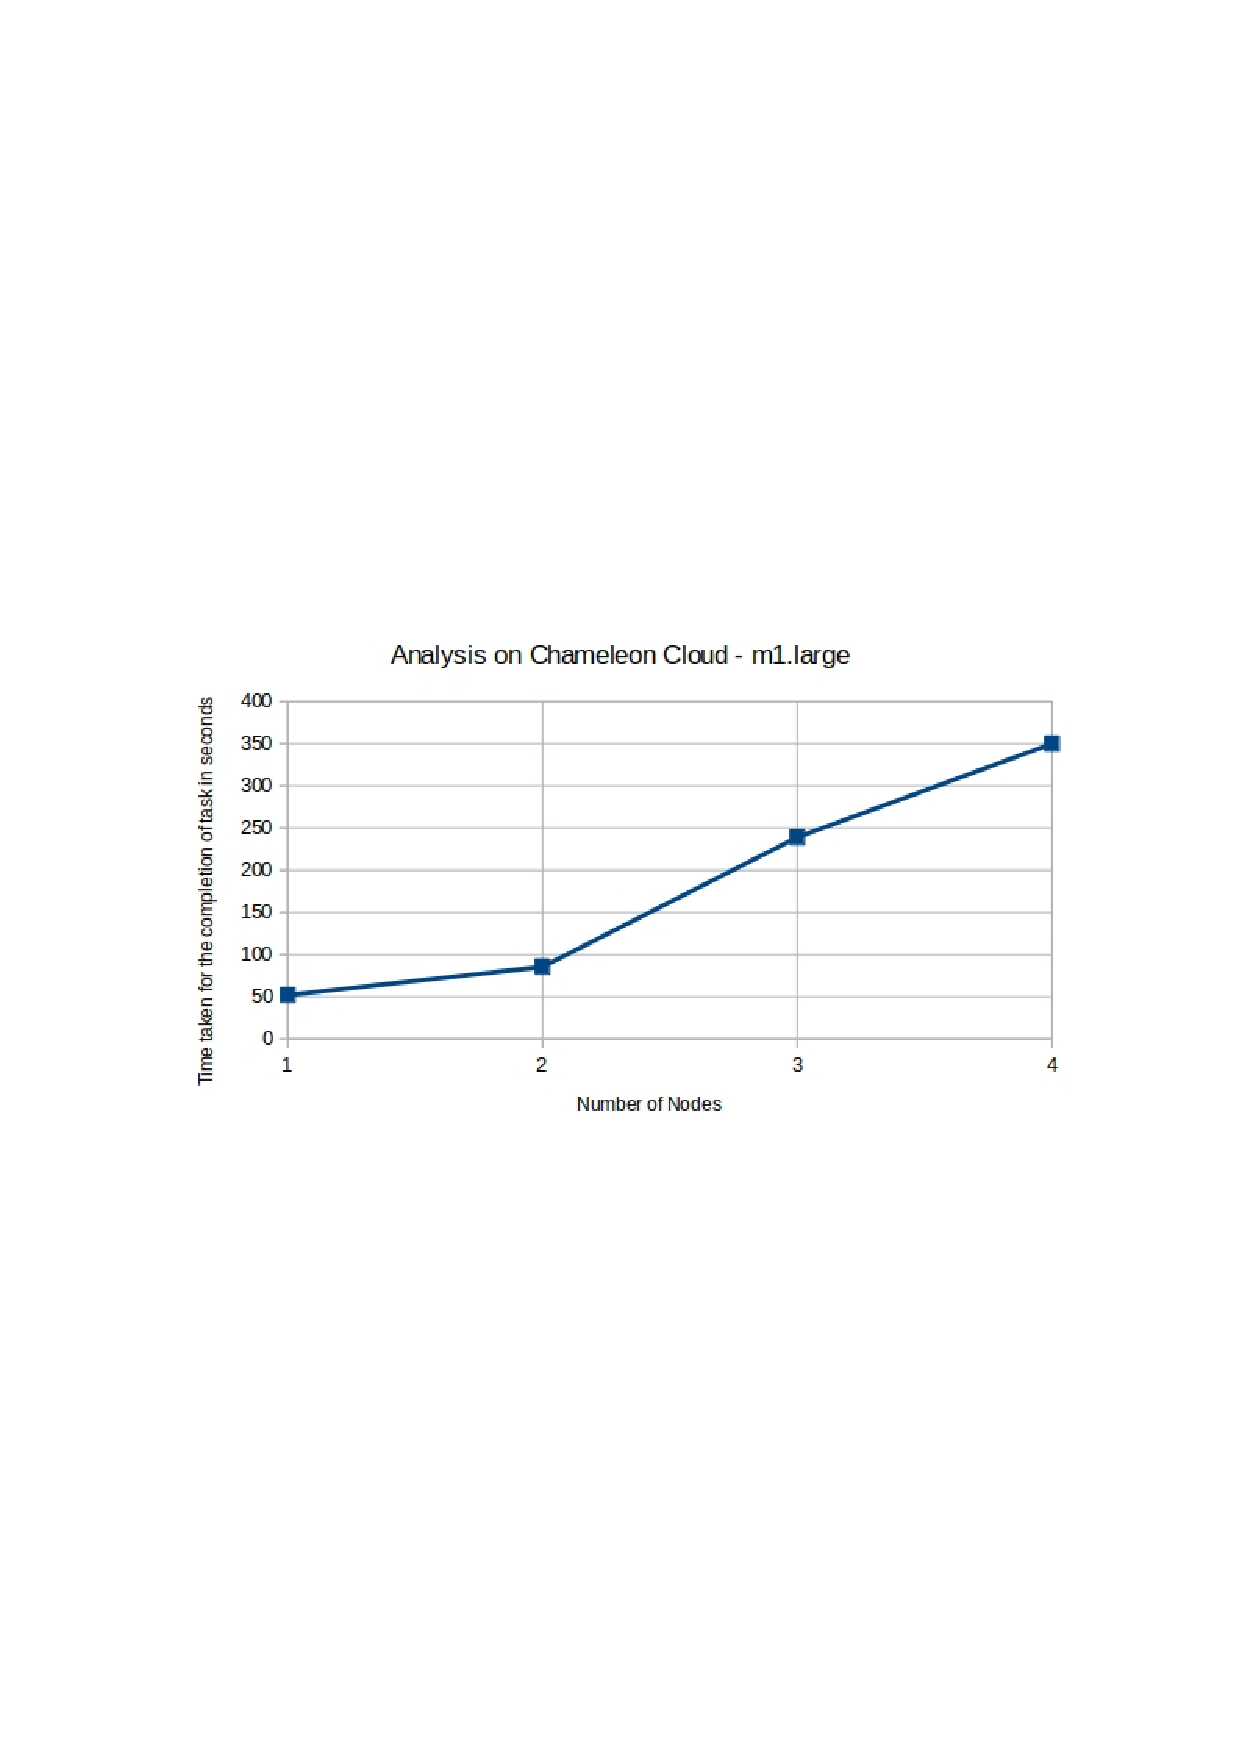
\includegraphics[width= \linewidth, height =
    2.5in]{images/m1large.pdf}
  \caption{Analysis time taken for a HiveQL-m1.large }
\end{figure}

\section{Conclusion}
Deployment and the analysis of the flight data is implemented by using
Apache Hive, Cloudmesh and Ansible automation. The results obtained
from the qeries in Hive environment gives insights on the available
flight data. Hive uses map and reduce functions internally which is
taken care of Hadoop system. Observations such as number of flights
cancelled, number of flights departed from an airport are made from
Hive Query Language. From these results trends and patterns are
observed which provide detailed analysis of the data.
\section{Acknowledgements}

This project is undertaken as part of the I524: Big Data and Open
Source Software Projects coursework at Indiana University. We would
like to thank our Prof. Gregor von Laszewski, Prof. Gregory Fox and
the Associate Instructors for their help and support.

\bibliography{references}

\end{document}
